\chapter{資料型態與描述性統計}
    在資料分析及統計推論前,我們經常需要先對資料有初步的認識,從而決定是否要先對資料做前處理(例如轉換、合併、處理離群值等等),以及應該用什麼統計方法進行分析。當資料量不大的時候,我們可以將資料全部列出來檢視,但隨著資料量的增大,我們就需要依賴描述性統計提取資料的特徵。本章我們將認識生醫資料常見的變數型態,針對這些變數型態有哪些適用的描述性統計量,以及這些描述性統計量的基本性質。
    
    \begin{introduction}[第 2 章學習目標]
        \item 生醫資料的變數常見型態
        \item 常見的描述性統計量及適用的變數型態
        \item 資料線性轉換對平均值、變異數、標準差的影響
    \end{introduction}

\section{生醫資料中變數的常見型態}

    一般生物醫學資料最常見的格式如下表:

    \begin{table}[htbp]
        \begin{center}
            \begin{tabular}{cccccccc}
                \toprule
                年齡 & 性別 & 教育程度 & 居住地 & 身高 & 體重 & 一年癲癇發作次數 & $\cdots$\\
                \hline
                30 & 男 & 高中(職) & 北北基 & 160 & 53.3 & 3 & $\vdots$ \\
                27 & 女 & 大專 & 中彰投 & 153 & 42.6 & 0 & $\vdots$ \\
                31 & 男 & 國中以下 & 桃竹苗 & 182 & 84.2 & 2 & $\vdots$ \\
                $\vdots$ & $\vdots$ & $\vdots$ & $\vdots$ & $\vdots$ & $\vdots$ & $\vdots$ & $\vdots$ \\
                \bottomrule
            \end{tabular}
            \caption{常見資料格式\label{tab:data}}
        \end{center}
    \end{table}
        
    其中每一個 row(橫列,但不同國家的行列定義不同,因此我們這裡通稱 row)代表一筆資料,也常被稱為一個\textit{觀察值} (observation)。每個 column(直行)則代表不同的測量標的,該標的也被稱為\textit{變數}或\textit{變項} (variable)。從表\ref{tab:data}可以看出,各變項依據其可能的取值可粗略分為兩種:一種是以類別名稱取值的\textit{類別型變項} (categorical variable),例如性別、教育程度、居住地;另一種則是以有實際意義的數字取值的\textit{數值型變項} (numerical variable),例如年齡、身高、癲癇發作次數。類別型變項的各種類別取值也被稱為\textit{層次} (level)。在實務上,為了節省資料存儲空間以及減少錯誤,類別型變項的取值常會被替換為整數的數字,例如性別為男取值 1、女取值 0,或是教育程度國中以下、高中(職)、大專、碩士、博士分別替換為0、1、2、3、4。替換的數字與層次實際名稱的對照表則存儲在編碼冊 (coding book) 中,如表\ref{tab:data_coding}所示。

    \newpage

    \begin{table}[htbp]
        \begin{center}
            \begin{tabular}{cccccccc}
                \toprule
                年齡 & 性別 & 教育程度 & 居住地 & 身高 & 體重 & 一年癲癇發作次數 & $\cdots$\\
                \hline
                30 & 1 & 1 & 1 & 160 & 53.3 & 3 & $\vdots$ \\
                27 & 0 & 2 & 3 & 153 & 42.6 & 0 & $\vdots$ \\
                31 & 1 & 0 & 2 & 182 & 84.2 & 2 & $\vdots$ \\
                $\vdots$ & $\vdots$ & $\vdots$ & $\vdots$ & $\vdots$ & $\vdots$ & $\vdots$ & $\vdots$ \\
                \bottomrule
            \end{tabular}

            \bigskip

            \begin{tabular}{c|l}
                \toprule
                性別 & 女:0;男:1\\
                \hline
                教育程度 & 國中以下:0;高中(職):1;大專:2;碩士:3;博士:4\\
                \hline
                \multirow{2}{*}{居住地} & 北北基:1;桃竹苗:2;中彰投:3;\\
                & 雲嘉南:4;高屏:5;宜花東:6;外島:7\\
                \bottomrule
            \end{tabular}
            \caption{常見編碼資料格式與編碼冊\label{tab:data_coding}}
        \end{center}
    \end{table}

    根據類別型變項和數字型變項的特性,我們還可以再將它們細分:

    \begin{itemize}
        \item 類別型變項
        \begin{itemize}
            \item \textit{名目} (Nominal):各層次間沒有排序關係的類別型變項,例如性別、居住地。
            \begin{itemize}
                \item \textit{二元} (Binary):僅有兩個層次的名目變項。為了後續分析方便,通常會把其中一個層次編碼為0,另一個層次編碼為1。
                \item \textit{多元} (Multinomial):有三個以上層次的名目變項。
            \end{itemize}
            \item \textit{有序} (Ordinal):各層次間有排序關係的類別型變項,例如教育程度、收入區間。為了後續分析方便,編碼通常會按照排序關係以遞增的整數編碼,如表\ref{tab:data_coding}的教育程度編碼。
        \end{itemize}
        \item 數值型變項
        \begin{itemize}
            \item \textit{計數} (Count):取值為非負的整數,例如一年內癲癇發生次數、牙齒剩餘顆數。
            \item \textit{連續} (Continuous):實務上如果取值不連續但是可能數值足夠多(例如身高均以整數紀錄、因此可能取值有限),常常也視為連續。
            \begin{itemize}
                \item \textit{等距} (Interval):變項取值的零點是人為的,因此兩個數值相除的意義不大。例如智商、pH 值。
                \item \textit{等比} (Ratio):變項取值有一個有意義的零點,使得兩個數值相除有意義。例如身高、體重。
            \end{itemize}
        \end{itemize}
    \end{itemize}

    \begin{custom}{思考}
        根據這個定義,攝氏溫度、華氏溫度和克式溫度(Kelvin scale)應該是哪種資料型態?如果一個問卷的題目讓填答者填1到5分的(整數)滿意度,那麼這個題目的答案應該是哪種資料型態?如果疼痛指數是1到10分的整數,那麼它應該是哪種資料型態?
    \end{custom}

    \begin{custom}{思考}
        如果資料是一張 X 光片,那麼我們還能把圖像轉成數值型態嗎?更進一步,如果圖像不是黑白的,那麼要怎麼轉成數值型態?
    \end{custom}

    \begin{custom}{思考}
        一般來說,資料中的每一個 row 通常代表一筆資料,而不同的 row 通常預設是由不同的病患所貢獻。如果我們現在追蹤一群高血壓病患十年,每三個月追蹤一次(共四十次),並想記錄他們追蹤起始年齡、性別、高血壓家族史及每次追蹤的收縮壓和舒張壓,那麼應該如何記錄資料?
    \end{custom}
    
\section{類別變項的描述性統計量}
    了解變項的資料型態後,我們就可以進一步探討如何選擇並計算描述性統計量,來描述變項的特徵。描述性統計量本質上還是一個參數估計量(請參見第一章),而且是用來估計母體描述性參數的估計量。因此我們要先探討針對各種資料型態的母體,有哪些適用的描述性參數,以及如何用樣本計算出描述性統計量來估計這些參數。

    對於類別變項最具描述性的參數,即為\textbf{各層次的出現比例}(由於類別變項各層次對應的編碼只是人為設定,所以一般來說,母體的描述性參數不會牽涉到這些編碼的數值。)。而估計這些比例的描述性統計量也很好計算,只要計算各層次在樣本中出現的比例即可。舉例而言,假設我們從清華大學隨機抽取了 100 位大學生並記錄了「性別」這個變項。我們的母體是清華大學的所有大學生,而這些大學生的性別層次有兩個:男和女,所以針對性別變項的母體描述性參數即為「清華大學生的男生比例」及「清華大學生的女生比例」(因為加起來等於一,所以知道一個比例就可以推出另外一個)。相對應的描述性統計量就是 100 位抽中的大學生中,男性和女性的比例。

\section{數值變項的描述性統計量}
    和類別變項不同的是,數值變項的取值可能性多了許多,而且具有解釋意義。因此數值變項的母體描述性參數相對於類別變項更為多元。針對數值變項,我們能用高中學到的直方圖來視覺化母體的取值狀況,如圖\ref{fig:descriptive_cont}所示。以下我們根據圖\ref{fig:descriptive_cont}討論一些常用的描述性參數。

    \begin{figure}[htbp]
      \centering
      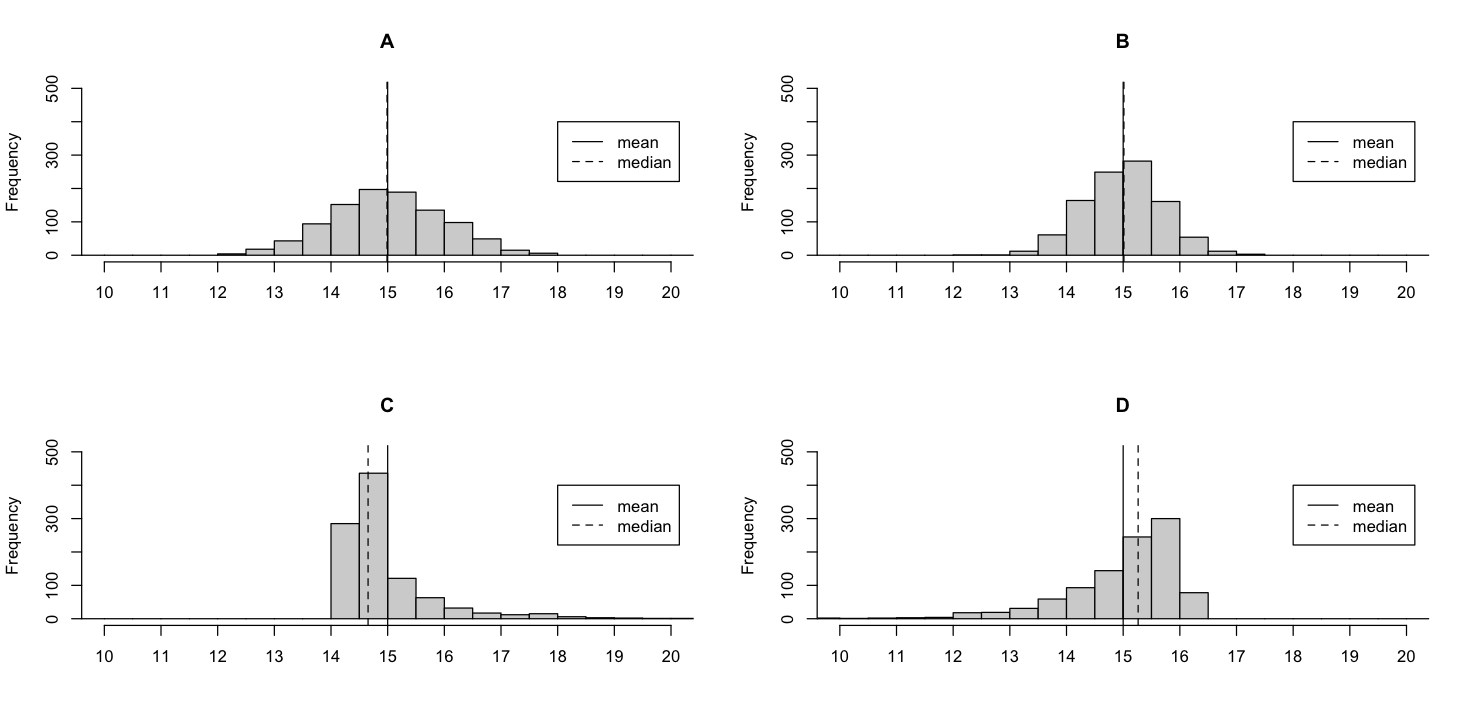
\includegraphics[width=\textwidth]{figures/02-Descriptive_statistics/descriptive_cont.png}
      \caption{四個不同母體的分布直方圖}
      \label{fig:descriptive_cont}
    \end{figure}

\subsection{位置參數及其描述統計量}
    描述變項母體分佈的第一步,通常是找尋它的中心位置,我們才知道可能的取值大多會落在哪個數值附近。描述母體中心位置的參數通常被稱謂\textit{位置參數} (location parameter)。其中最常見的位置參數就是我們耳熟能詳的\textit{平均值} (mean),或是更精準的一點說,\textit{算術平均值} (population arithmetic mean)。假設變項 $X$ 的母體有 $N$ 個觀察值,分別為 $\tilde{X}_1, \tilde{X}_2, ... \tilde{X}_N$,則 $X$ 的\textit{母體平均} $\mu_X$ 的定義為:
    \[\mu_X = \frac{\tilde{X}_1+\tilde{X}_2+\cdots+\tilde{X}_N}{N} = \frac{1}{N}\sum_{i=1}^N \tilde{X}_i\]
    估計母體平均值的描述統計量被稱為\textit{樣本平均} (sample mean),常簡寫為 $\bar{X}$(唸作 X bar),假設樣本數為 $n$,觀察值分別為$X_1, X_2, ... X_n$,則樣本平均 $\bar{X}$ 的定義很直觀:
    \[\bar{X} = \frac{X_1+X_2+\cdots+X_n}{n} = \frac{1}{n}\sum_{i=1}^n X_i\]
    也就是把樣本觀察值全部加總取平均。注意到如果把變項做線性的放大平移 $X^* = aX+b$ ,也就是將放大$a$倍後加上$b$,那麼新的母體平均和樣本平均 $\mu_X^*$ 和 $s_X^2$ 會變成:
    \begin{align*}
        \mu_X^* &= \frac{(a\tilde{X}_1+b)+(a\tilde{X}_2+b)+\cdots+(a\tilde{X}_N+b)}{N}\\
        &= \frac{a(\tilde{X}_1+\tilde{X}_2+\cdots+\tilde{X}_N)+Nb}{N}\\
        &= a\frac{\tilde{X}_1+\tilde{X}_2+\cdots+\tilde{X}_N}{N} + \frac{Nb}{N} = a\mu_X + b\\
        \bar{X}^* &= \frac{(aX_1+b)+(aX_2+b)+\cdots+(aX_n+b)}{n}\\
        &= \frac{a(X_1+X_2+\cdots+X_n)+nb}{n}\\
        &= a\frac{X_1+X_2+\cdots+X_n}{n}+\frac{nb}{n}=a\bar{X}+b
    \end{align*}
    所以平均值同樣會以相同的倍率放大平移。
    
    平均值的算法雖然簡單,但是它的數值很容易受到極端的觀察值影響而偏移。例如在圖\ref{fig:descriptive_cont}的 C 中,雖然大於七成的母體取值都落在 14 到 15 之間,但母體平均值受到右方較大的數值影響而被往右拉到 15。此處以平均值 15 當作母體分布的「中心」似乎就不太合理。\textit{中位數} (median)是解決這個問題的一個替代方案,它的想法是把所有的取值由小排到大,並選取位置在正中間的數值。如果取值的數目為偶數,則取最中間兩個數值的平均。換句話說,如果把變項 $X$ 的母體觀察值由小排到大得到 $\tilde{X}_{(1)}, \tilde{X}_{(2)}, ..., \tilde{X}_{(N)}$,則母體中位數 $M_X$ 的定義為:
    \[M_X = \left\{\begin{array}{lr}
        \tilde{X}_{(\frac{N+1}{2})}, & N \text{是奇數}\\
        \frac{1}{2}\Big[\tilde{X}_{(\frac{N}{2})}+\tilde{X}_{(\frac{N}{2}+1)}\Big], & N \text{是偶數}
    \end{array}\right.\]
    估計母體中位數的描述性統計量即為\textit{樣本中位數} (sample median),其定義一樣很直觀:假設樣本觀察值由小排到大分別為$X_{(1)}, X_{(2)}, ... X_{(n)}$,則樣本中位數 $\hat{M}_X$ 為:
    \[\hat{M}_X = \left\{\begin{array}{lr}
        X_{(\frac{N+1}{2})}, & N \text{是奇數}\\
        \frac{1}{2}\Big[X_{(\frac{N}{2})}+X_{(\frac{N}{2}+1)}\Big], & N \text{是偶數}
    \end{array}\right.\]
    如前所述,中位數雖然常和平均值相去不遠,但是當變項的分布在一個方向有較多的極端值時,中位數就會和平均值有差距。如果極端值較常出現在右側,我們稱該分布為\textit{右偏} (right-skewed)或\textit{正偏} (positively skewed),此時一般而言,中位數會比平均值來得小(如圖\ref{fig:descriptive_cont}的C)。反之,如果極端值較常出現在左側,我們稱該分布為\textit{左偏} (left-skewed)或\textit{負偏} (negatively skewed),此時一般而言,中位數會比平均值來得大(如圖\ref{fig:descriptive_cont}的D)。
    
    雖然中位數雖然的確能夠直指分布的「中心」,但它的統計性質較為複雜,在後續很多的推論統計方法沒有辦法直接適用,因此一般而言我們還是會優先選擇平均值作為我們的位置參數以及描述統計量。另外一個可用的位置參數是 \textit{眾數} (mode),也就是所有觀察值中出現頻率最高的數值。不過在數值型變項,尤其是連續型變項中,各樣本取值的頻率常常都很低(例如一群人中,體重數值如果取到小數點後一位,那麼每種可能取值的出現次數可能都只有一次),所以實務上不常使用。

    \begin{custom}{思考}
        如果某個變項在收集的過程中,已經先行將連續的變項分割為多個區間,並且記錄區間的頻率(例如 10-20 歲多少人、20-30 歲多少人、40-50 歲多少人),那麼我們還有辦法對該變項計算位置相關的描述統計量嗎?
    \end{custom}

\subsection{分散參數及其描述統計量}
    除了位置參數以外,我們看到 A 和 B 兩個變項的母體平均值和中位數均為 15 ,但是 B 的可能取值跨度明顯地比 A 還要小。換句話說,相對於 A,B 的取值比較常落在離平均值比較近的位置。用來描述這個分布特性的參數稱為分散參數 (dispersion parameter)。
    
    一個變項的取值和平均值之間的距離,如果平均而言較遠(例如圖\ref{fig:descriptive_cont}中的 A 有為數不少的取值跟平均值 15 的距離大於 1),那麼這個變項的分散程度應該比較大。因此,直覺上分散參數的定義可以用「取值和平均值的平均距離」來定義。如此定義的分散參數稱為\textit{平均絕對離差} (mean absolute deviation),也就是:
    \[\text{MAD}_X = \frac{|\tilde{X}_1-\mu_X|+|\tilde{X}_2-\mu_X|+\cdots+|\tilde{X}_N-\mu_X|}{N} = \frac{1}{N} \sum_{i=1}^N |\tilde{X}_i-\mu_X|\]

    雖然平均絕對離差的定義很符合直覺,但是它含有絕對值,處理起來較為複雜。因此,統計學中較常使用的分散參數定義為「取值和平均值之平方距離的平均」。如此定義的分散參數即為著名的\textit{變異數} (variance),通常記為$\sigma^2_X$。以符號定義母體變異數 (population variance) 如下:
    \[\sigma^2_X = \frac{(\tilde{X}_1-\mu_X)^2+(\tilde{X}_2-\mu_X)^2+\cdots+(\tilde{X}_N-\mu_X)^2}{N} = \frac{1}{N} \sum_{i=1}^N (\tilde{X}_i-\mu_X)^2\]
    估計母體變異數的描述性統計量稱為\textit{樣本變異數} (sample variance),通常以 $s^2_X$ 代表。按照前面平均值和中位數的經驗,樣本變異數應該直接把母體觀察值 $\tilde{X}_i$ 換成樣本觀察值 $X_i$。但是這樣還不夠,因為我們不知道母體平均數 $\mu_X$ 的值,所以需要用樣本平均數 $\bar{X}$ 來估計代換 $\mu_X$,而得到下面的式子:
    \[\frac{(X_1-\bar{X})^2+(X_2-\bar{X})^2+\cdots+(X_n-\bar{X})^2}{n}\]
    很不幸地,上述的樣本估計式會\textbf{低估}母體變異數。我們可以用圖\ref{fig:degrees_of_freedom}來獲得一個直覺的解釋。當我們抽樣都抽到數值較小的觀察值時(如圖\ref{fig:degrees_of_freedom}中的四個紅點),母體變異數的定義希望我們計算觀察值到\textbf{母體平均}的平方距離,此時母體平均比樣本觀察值都來得大(圖\ref{fig:degrees_of_freedom}的實線),但是這個估計式是計算觀察值到\textbf{樣本平均}的平方距離,而樣本平均基本上會在樣本觀察值的中心(圖\ref{fig:degrees_of_freedom}的虛線)。因此,估計式計算出的平方距離會比母體變異數想要計算的來得小。同樣的,如果抽樣都抽到數值較大的觀察值,也是會有低估的狀況。解決的方法是對分母做一個校正:除以樣本數減一($n-1$)而不是樣本數。至於為何是樣本數減一而不是減其他數,我們會在後續的課程做說明,這裡就暫且假設下述的定義是較佳的樣本變異數計算方法:
    \[s^2_X = \frac{(X_1-\bar{X})^2+(X_2-\bar{X})^2+\cdots+(X_n-\bar{X})^2}{n-1} = \frac{1}{n-1} \sum_{i=1}^n (X_i-\bar{X})^2\]

    \begin{figure}[htbp]
      \centering
      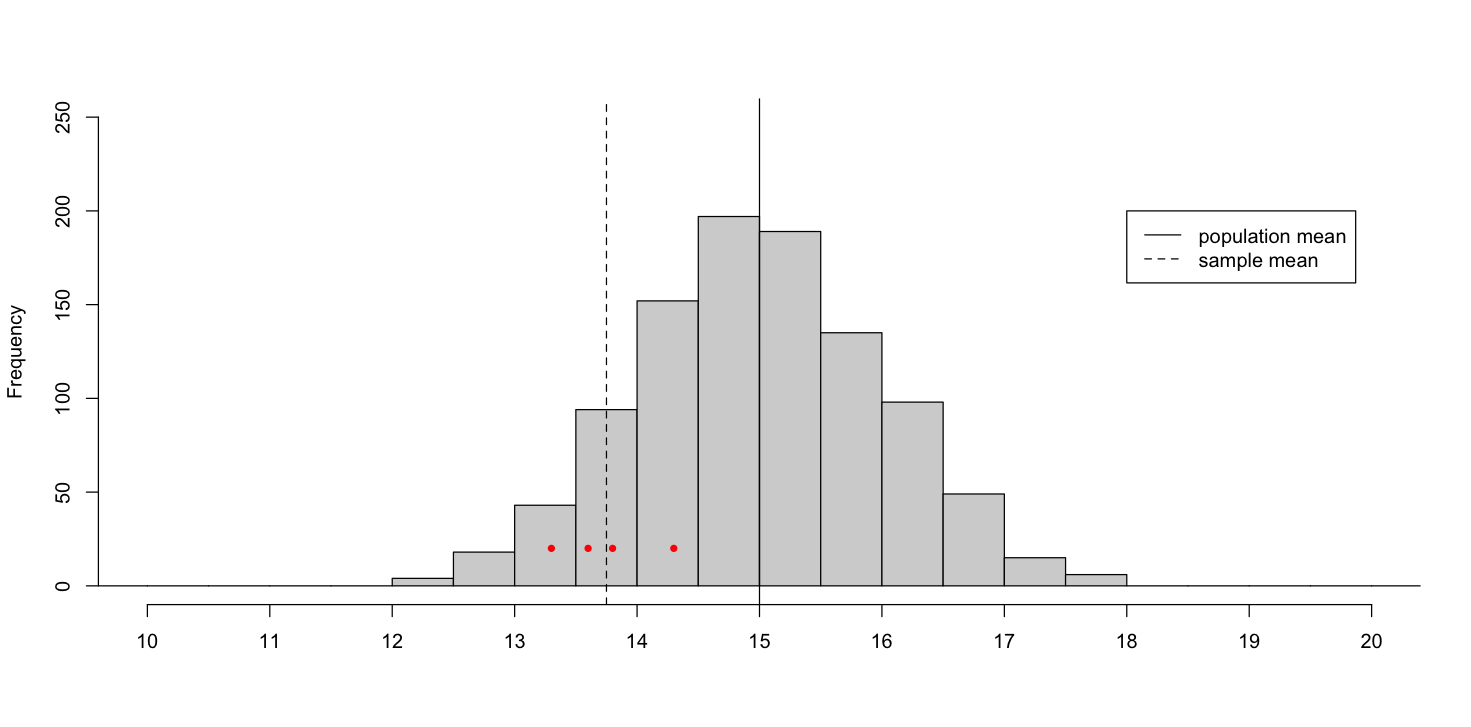
\includegraphics[width=\textwidth]{figures/02-Descriptive_statistics/degrees_of_freedom.png}
      \caption{估計母體變異數的低估問題}
      \label{fig:degrees_of_freedom}
    \end{figure}

    變異數雖然是一個很好用的分散參數,但如果仔細思考它的定義,會發現因為它是對「取值和母體平均之差值」的平方取平均,所以變異數的單位會是該變項單位的平方。例如,如果變項是收縮壓,單位是mmHg,那麼變異數的單位就會是$\text{mmHg}^2$,造成我們解釋上的困難。因此,我們再定義一個變異數的開根號為\textit{標準差} (standard deviation),作為一個新的分散參數。母體標準差通常寫作$\sigma_X$,其符號定義如下:
    \[\sigma_X = \sqrt{\frac{(\tilde{X}_1-\mu_X)^2+(\tilde{X}_2-\mu_X)^2+\cdots+(\tilde{X}_N-\mu_X)^2}{N}} = \sqrt{\frac{1}{N} \sum_{i=1}^N (\tilde{X}_i-\mu_X)^2}\]
    而估計母體標準差的樣本估計量稱為樣本標準差,通常記做$s$,其符號定義也十分直覺:
    \[s_X = \sqrt{\frac{(X_1-\bar{X})^2+(X_2-\bar{X})^2+\cdots+(X_n-\bar{X})^2}{n-1}} = \sqrt{\frac{1}{n-1} \sum_{i=1}^n (X_i-\bar{X})^2}\]
    (註:理論上上述的樣本標準差還要再進行校正才會成為母體標準差的最佳估計方法,但實務上差異不大且太過複雜,所以大多使用上述的簡單公式。)

    標準差的單位和原變項相同,因此可以看成是分布「寬度」的一個指標。若將其與平均值的組合,可以讓我們對變項做最初步的了解。在母體分布不要太奇形怪狀的情況下,我們可以套用經驗性的「68-95-99.7法則」:
    \begin{itemize}
        \item 母體約有$68\%$的取值會在 $\mu-\sigma$ 與 $\mu+\sigma$ 之間
        \item 母體約有$95\%$的取值會在 $\mu-2\sigma$ 與 $\mu+2\sigma$ 之間
        \item 母體約有$99.7\%$的取值會在 $\mu-3\sigma$ 與 $\mu+3\sigma$ 之間
    \end{itemize}
    因此,如果資料中出現離平均值兩倍標準差、甚至三倍標準差以外的觀察值,就可以進一步調查該觀察值,是否有測量錯誤的問題。
    
    如同之前在平均值的討論,我們也可以探討變項如果做線性的放大平移,會對變異數和標準差造成什麼影響。首先,直覺上,因為平移變項的數值並不會改變其分散程度,所以平移不應該改變變異數及標準差。我們可以簡單地驗證:假設我們對變項 $X$ 做平移得到 $X^* = X+b$,則我們已知母體平均數會變成 $\mu_X^* = \mu_X+b$,所以新的母體變異數為:
    \begin{align*}
        \sigma^{2*}_X &= \frac{[(\tilde{X}_1+b)-(\mu_X+b)]^2+[(\tilde{X}_2+b)-(\mu_X+b)]^2+\cdots+[(\tilde{X}_N+b)-(\mu_X+b)]^2}{N} \\
        &= \frac{[\tilde{X}_1-\mu_X]^2+[\tilde{X}_2-\mu_X]^2+\cdots+[\tilde{X}_N-\mu_X]^2}{N} = \sigma_X^2
    \end{align*}
    同樣地,樣本變異數也不會受到平移的影響。由於標準差為變異數開根號,所以也不會受到平移的影響。

    假設我們並非對變項 $X$ 做平移,而是縮放而得到 $X^* = aX$,例如把 $X$ 的測量單位從公尺變成公分,使得數值變為 100 倍,則我們已知母體平均數會變成 $\mu_X^* = a\mu_X$,所以新的母體變異數為:
    \begin{align*}
        \sigma^{2*}_X &= \frac{(a\tilde{X}_1-a\mu_X)^2+(a\tilde{X}_2-a\mu_X)^2+\cdots+(a\tilde{X}_N-a\mu_X)^2}{N} \\
        &= a^2\frac{(\tilde{X}_1-\mu_X)^2+(\tilde{X}_2-\mu_X)^2+\cdots+(\tilde{X}_N-\mu_X)^2}{N} = a^2\sigma_X^2
    \end{align*}
    因此,縮放後,母體變異數會以平方的倍數被縮放。同樣地,樣本變異數也會被平方的倍數縮放。由於標準差為變異數開根號,所以標準差的縮放倍數會和變項的縮放倍數大小相同(需加上絕對值),也就是$\sigma^*_X = a\sigma_X$。

    除了變異數和標準差外,\textit{全距} (range) 和 \textit{四分位差} (interquartile range) (尤其是四分位差)也會被拿來作為量化變數分散程度的描述統計量。全距的定義十分直觀,即為最大觀察值和最小觀察值之差,不過也因此全距非常容易受到極端值的影響,對於分散程度的量化效果不如其他統計量。四分位差則牽涉到百分位數的計算。我們之前計算過的中位數其實就是第 $50$ 百分位數,而第 $p$ 百分位數的計算方式為($\lceil.\rceil$為取比括號內大的最小整數)
    \[\left\{\begin{array}{lr}
        X_{(\lceil np/100 \rceil)}, & np/100 \text{非整數}\\
        \frac{1}{2}\Big[X_{(np/100)}+X_{(np/100+1)}\Big], & np/100 \text{為整數}
    \end{array}\right.\]
    第一、第二、第三四分位分別為變項的第 25、50、75 百分位數,而四分位差的定義則為第三四分位與第一四分位的差。由此可以看到,四分位差不會受到數值最大和最小 25$\%$ 資料的影響,對於極端值較不敏感。因此在實務上,如果資料分布有較多的極端值,如圖\ref{fig:descriptive_cont}中的C和D,可以考慮以四分位差取代標準差作為分散程度的指標。

    \begin{custom}{思考}
        如果對資料作線性的放大平移,那麼中位數、全距和四分位差應該會如何變動?
    \end{custom}